\section{Decay (Damping) of Free Oscillations}

In general, resistive forces act in a direction opposite to $\vec{v}$ and have magnitude:
\[ F_b = b_1v + b_2v^2\]

When $v$ is small in comparison to $b_1/b_2$, we can make an approximation:
\begin{equation*}
	\boxed{\vec{F}_b = -b\vec{v}}
\end{equation*}

If our mass-spring system (cf. Section~\ref{ch3:sec-simple-springs}) had damping, our statement of Newton's Law would have been:
\begin{align}
	m\ddot{x} &= -kx - bv \notag \\
	m\ddot{x} + b\dot{v} + kx &= 0 \notag  \\
	\Aboxed{\ddot{x} + \gamma \dot{x} + \omega_0^2 x &= 0} \label{ch3:eq-damping-NL}
\end{align}
where
\[ \boxed{\gamma = \frac{b}{m} \andd \omega_0^2 = \frac{k}{m}} \]

Interpretation:
\begin{itemize}
	\item $\gamma$: damping constant (with dimensions of frequency)
	\begin{itemize}
		\item We will also that see it represents the reciprocal of the time required for the energy to decrease to $1/e$ of its initial value (Section~\ref{ch3:sec-quality-factor})
	\end{itemize}
	\item $\omega_0$: angular frequency of the system if \emph{damping were absent}
\end{itemize}

The solution to \eqref{ch3:eq-damping-NL} when there is \textbf{underdamping} $(\omega_0>\gamma/2)$ is:
\begin{equation}
	\boxed{
		x = A_0 e^{-\gamma t/2} \cos(\omega t + \alpha) \where \omega ^2 = \omega_0^2 - \frac{\gamma^2}{4} 
	}	\label{ch3:eq-damping-solution}
\end{equation}

We can interpret $\omega$ as the angular frequency of the \emph{damped oscillator}.


\subsection{Underdamping $(\omega_0 > \gamma/2)$}
\begin{proof}[Solving for the equation of motion]
	Assume $x$ is the real part of a rotating vector $z$. So:
	\begin{equation*}
		\ddot{z} + \gamma \dot{z} + \omega_0^2 z = 0
	\end{equation*}
	
	Assume the following solution\footnote{Note that this assumed solution contains two constants -- this takes into account that \eqref{ch3:eq-damping-NL} is a second-order differential equation.}:
	\begin{equation}
		z=A_0 e^{j(pt+\alpha)} \label{ch3:eq-damping-assumed-z}
	\end{equation}
	
	Substitute to obtain:
	\begin{align}
		(A_0 j^2 p^2 e^{j(pt+\alpha)}) + \gamma (A_0 jpe^{j(pt+\alpha)}) + \omega_0^2 (A_0 e^{j(pt+\alpha)}) &= 0 \notag \\
		A_0 e^{j(pt+\alpha)}(-p^2 + jp \gamma + \omega_0^2) &= 0 \notag \\
		\Longrightarrow (-p^2 + jp \gamma + \omega_0^2) &= 0 \label{ch3:eq-damping-pj}
	\end{align}
	
	$p$ cannot be a purely real number -- if that were the case, $jp\gamma$ would not get cancelled. So, assume:
	\begin{equation} 
		p = n + js \where \text{$n,s$ are real} \label{ch3:eq-damping-p}
	\end{equation}
	\[ \Longrightarrow p^2 = n^2 + 2jns - s^2 \]
	
	Substitute into \eqref{ch3:eq-damping-pj}:
	\begin{align}
		(-(n^2 + 2jns - s^2) + j \gamma (n+js) + \omega_0^2) &= 0 \notag \\
		-n^2 - 2jns + s^2 + nj \gamma - s \gamma + \omega_0^2 &= 0 \notag \\
		\underbrace{(-n^2 + s^2  - s \gamma + \omega_0^2)}_\text{real part} +  \underbrace{j(-2ns + n \gamma)}_\text{imaginary part} &= 0 \label{ch3:eq-damping-real-imag}
	\end{align}
	
	Both the real and the imaginary parts of \eqref{ch3:eq-damping-real-imag} must equal zero:
	\begin{align*}
		\text{Real part: } \htab & -n^2 + s^2  - s \gamma + \omega_0^2 = 0 \\
		\text{Imaginary part: } \htab &-2ns + n \gamma = 0 
	\end{align*}
	
	From the imaginary part,
	\[ s=\frac{\gamma}{2}\]
	Substitute this into the real part to obtain:
	\[ n^2 = \omega_0^2 - \frac{\gamma^2}{4} \]
	
	Returning to our assumed solution for $z$ \eqref{ch3:eq-damping-assumed-z}, substitute in our expressions for $s$ and $n$:
	\begin{align*}
		z&=A_0 e^{j((n+js)t+\alpha)}  \\
		z &= A_0 e^{-st} e^{j(nt+\alpha)} \\
		z &= A_0 e^{-st} [ \cos(nt+\alpha) + j\sin(nt+\alpha)  ]
	\end{align*}
	\[ 	\Longrightarrow x = \Re(z) = A_0 e^{-st}\cos(nt+\alpha) \]
	\[ \therefore 
	x = A_0 e^{-\gamma t/2} \cos(\omega t+\alpha) \where \omega^2 = \omega_0^2 - \frac{\gamma^2}{4} \]
\end{proof}


\begin{figure}
	\centering
	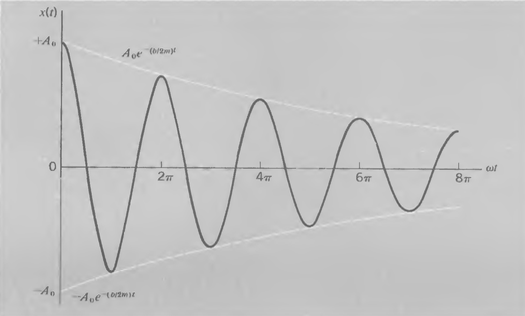
\includegraphics[scale=0.55]{phys232/Ch3-underdamping.png} \caption{Rapidly underdamped harmonic oscillations.}\label{ch3:fig-underdamping}
\end{figure}

Our solution \eqref{ch3:eq-damping-solution} is plotted in Figure~\ref{ch3:fig-underdamping}. Notice that:
\begin{itemize}
	\item A half-period $(\Delta t = \pi/2)$ elapses between zeroes, as well as between successive maxima and minima.
	\item However, the extrema are now only \emph{approximately halfway} between the zeroes.
\end{itemize}

\paragraph{Very Small Damping $(\gamma \ll \omega)$}

When the damping is very small, the motion approximates to SHM at a constant amplitude over a number of cycles around time $t$.

Amplitude around time $t$:
\[ A(t) = A_0 e^{-\gamma t/2} \]

Total energy around time $t$:
\begin{align*}
	E(t) = \frac{1}{2}kA^2 
	&= \frac{1}{2}kA_0^2 e^{-\gamma t} \\
	\Aboxed{\therefore E(t) &= E_0 e^{-\gamma t} }
\end{align*}
i.e. the total energy decays exponentially.

\paragraph{Quality Factor} \label{ch3:sec-quality-factor}
We can also interpret $\gamma$ as representing the reciprocal of the time required for the energy to decrease to $1/e$ of its initial value. Let us examine why.

We can define a \textbf{quality value} to describe the amount of damping:
\begin{equation}
	\boxed{Q = \frac{\omega_0}{\gamma}} 
	\so 
	\gamma = \frac{\omega_0}{Q}
	\label{ch3:eq-Q-def}
\end{equation}

We can rewrite \eqref{ch3:eq-damping-solution} in terms of $Q$:
\begin{equation}
	\omega^2 = \omega_0^2 \left(1- \frac{1}{4Q^2}\right) \label{ch3:eq-damping-sol-with-Q}
\end{equation}

\eqref{ch3:eq-damping-sol-with-Q} implies that for large $Q$ (i.e. as $Q \to \infty$), $\omega \to \omega_0$. 
Combining \eqref{ch3:eq-Q-def} with \eqref{ch3:eq-damping-solution} gives:
\[ x = A_o e^{-\omega_0 t/2Q} \cos(\omega_0 t + \alpha) \]
\[ \Longrightarrow A(t) = A_o e^{-\omega_0 t/2Q} \]

Re-express $t$ in terms of the number of cycles $n$. We have:
\[ t = \frac{2\pi n}{\omega} \approx \frac{2\pi n}{\omega_0} \]
\[ \Longrightarrow A(n) \approx A_0 e^{-n\pi/Q} \]

Therefore, for the amplitude to fall to $A_0/e$, we need $Q/\pi$ cycles of oscillation.

\paragraph{Another rewriting we can do}
Because $\gamma=\omega_0/Q$ \eqref{ch3:eq-Q-def}, \eqref{ch3:eq-damping-NL} becomes:
\[ \boxed{ \ddot{x} + \frac{\omega_0}{Q}\dot{x} + \omega_0^2 x = 0 } \]


\subsection{Overdamping ($ \omega_0 < \gamma/2 $)}

\begin{figure}
	\centering
	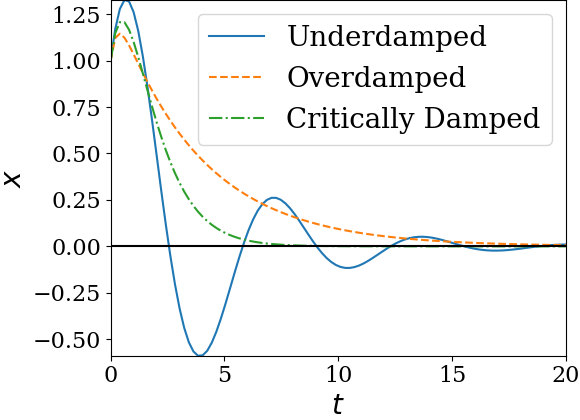
\includegraphics[scale=0.6]{phys232/Ch3-damped-oscillators-graph.png} \caption{Three cases of damping: (a) underdamping $(\omega_0>\gamma/2)$; (b) overdamping $(\omega_0<\gamma/2)$; (c) critical damping $(\omega_0=\gamma/2)$} \label{ch3:fig-damping}
\end{figure}


The motion is no longer oscillatory -- see Figure~\ref{ch3:fig-damping}b.

Recall that the solution to \eqref{ch3:eq-damping-NL} was of the form:
\[ 	x = \Re\left[ A_0 e^{-\gamma t/2} e^{j(\omega t+\alpha)} \right] \]
where
\[ \omega^2 = \omega_0^2 - \frac{\gamma^2}{4} \]
\[ \Longrightarrow \omega^2 =  -\left( \frac{\gamma^2}{4} - \omega_0^2 \right)  \]

Solving for $\omega$:
\[ \omega = \pm j\sqrt{ \frac{\gamma^2}{4}-\omega_0^2  } = \pm j\beta \]

Because of the two possibilities for $\omega$, we can write our solution more generally as%
\footnote{This is the same reasoning we used to obtain the ``more-general" solution in \eqref{ch3:eq-complex-general-sol}}:
\[ \boxed{ \therefore
	x = A_1 e^{-(\gamma/2 + \beta)t} + A_2 e^{-(\gamma/2-\beta)t} 
	\where \beta = \sqrt{\frac{\gamma^2}{4}-\omega_0^2} 
} \]

Note that $\beta$ is only defined when $\omega_0^2 < \gamma^2/4$.

\subsection{Critical Damping ($ \omega_0 = \gamma/2 $)}
\[ \boxed{x = (A + Bt) e^{\gamma t/2}} \]

When a force is applied to a critically damped system at rest, there will be a smooth approach to a new equilibrium position without oscillation or overshoot -- see Figure~\ref{ch3:fig-damping}c.